\subsection{M.PC.PV - Planned Value e M.PC.EV - Earned Value}
\label{sec:PV&EV}

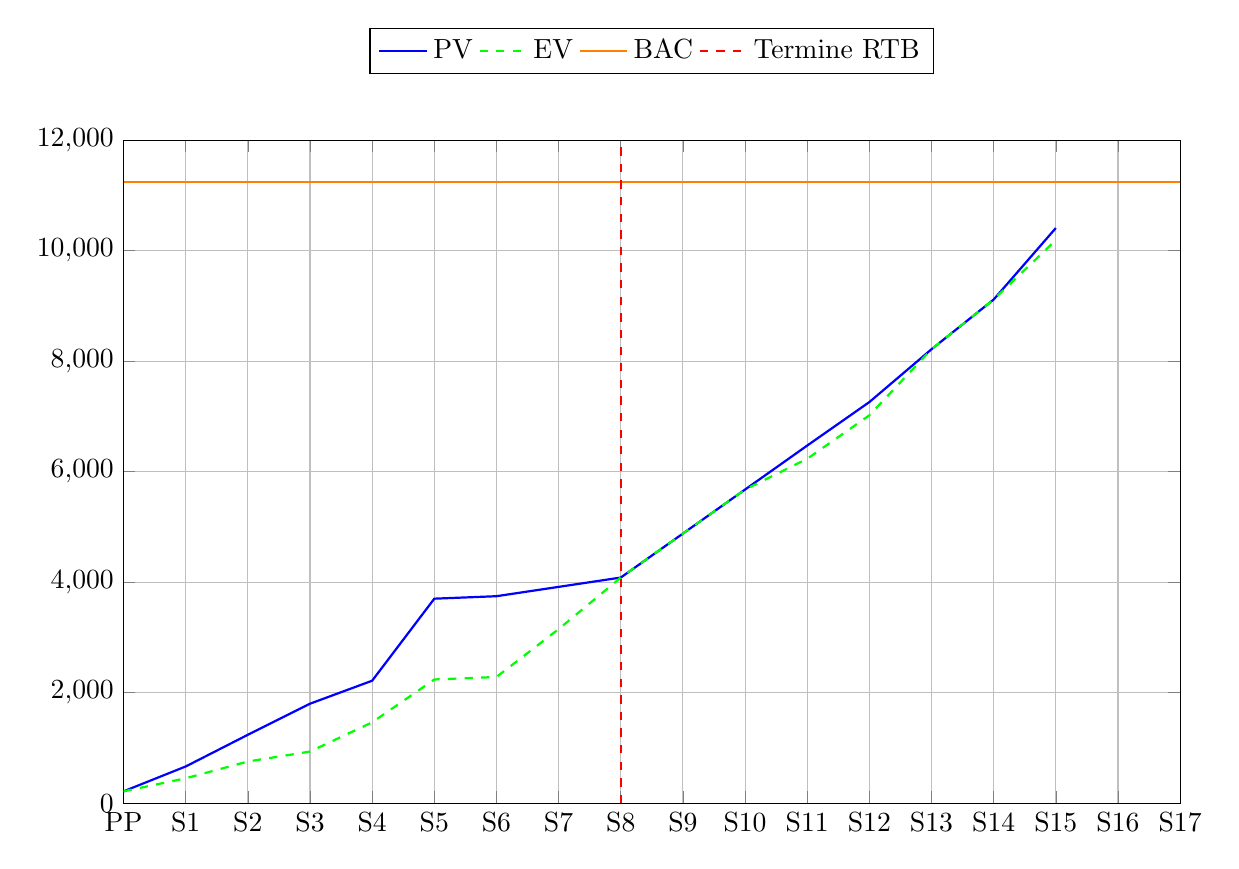
\begin{tikzpicture}
    \begin{axis}[
        width=15cm, height=10cm,
        ymin=0, ymax=12000,
        xmin=0, xmax=17,
        xtick={0, 1, 2, 3, 4, 5, 6, 7, 8, 9, 10, 11, 12, 13, 14, 15, 16, 17, 18},
        xticklabels={PP, S1, S2, S3, S4, S5, S6, S7, S8, S9, S10, S11, S12, S13, S14, S15, S16, S17, S18},
        xlabel={},
        ylabel={},
        grid=major,
        scaled ticks=false,
        legend style={at={(0.5,1.1)}, anchor=south, legend columns=-1},
    ]
    \addplot[color=blue, thick] coordinates {(0, 213.75) (1, 663.75) (2, 1237.5) (3, 1800) (4, 2216.25) (5, 3701.25) (6, 3746.25) (7, 3915) (8, 4083.75) (9, 4880.25) (10, 5676.75) (11,6473.25) (12,7260.75) (13, 8217) (14, 9117) (15, 10410.75)};
    \addlegendentry{PV}
    \addplot[color=green, thick, dashed] coordinates {(0, 213.75) (1, 450) (2, 753.75) (3, 933.75) (4, 1462.5) (5, 2238.75) (6, 2283.75) (7, 3150) (8, 4083.75) (9, 4880.25) (10, 5676.75) (11,6233.75) (12,7021) (13, 8217) (14, 9117) (15, 10191.375)};
    \addlegendentry{EV}
    \addplot[orange, thick] coordinates {(0, 11250) (17, 11250)};
    \addlegendentry{BAC}
    \addplot[red, thick, dashed] coordinates {(8, 0) (8, 12000)};
    \addlegendentry{Termine RTB}
    \end{axis}
\end{tikzpicture}
\subsubsection{RTB}
Come visibile dal grafico l'\glossario{Earned Value} è sempre inferiore rispetto al \glossario{Planned Value}, indicando una pianificazione 
mal riuscita da parte del gruppo.

\paragraph{Sprint 9}
Suddividendo la percentuale di lavoro rimanente fino al termine del progetto per ogni \glossario{sprint}, il gruppo ha pianificato di completare almeno il 7.08\% del lavoro totale per ogni \glossario{sprint}.
Poiché sono state completate tutte le \glossario{issue} preventivate per lo \glossario{Sprint} 9 il valore dell'\glossario{EV} risulta uguale al valore del \glossario{PV}.

\paragraph{Sprint 10}
Poiché sono state completate tutte le \glossario{issue} preventivate per lo \glossario{Sprint} 10 il valore dell'\glossario{EV} risulta uguale al valore del \glossario{PV}.

\paragraph{Sprint 11}
Non sono state completate tutte le \glossario{issue} preventivate per lo \glossario{Sprint} 11, ciò ha comportato la diminuzione del valore dell'\glossario{EV} a 4.956\% rispetto al 7.08\% del \glossario{PV} preventivato.

\paragraph{Sprint 12}
Sono state completate tutte le \glossario{issue} preventivate per lo \glossario{Sprint} 12. Il valore dell'\glossario{EV} risulta dunque uguale al 7\% invece del 7.08\% visto che erano stato preventivate 35 ore invece delle 39 previste per ogni sprint.

\paragraph{Sprint 13}
Sono state completate tutte le \glossario{issue} arretrate e tutte le \glossario{issue} pianificate per lo \glossario{sprint}, perciò il valore dell'\glossario{EV} risulta equivalente a quello del \glossario{PV}.
Siccome erano state pianificate 55 ore di lavoro l'aumento nel valore pianificato totale è di 9.6\% invece che del 7.08\%, considerato l'aumento medio necessario per terminare nei tempi il progetto.

\paragraph{Sprint 14}
Sono state completate tutte le \glossario{issue} pianificate per lo \glossario{sprint}, perciò il valore dell'\glossario{EV} risulta equivalente a quello del \glossario{PV}.
Siccome erano state pianificate 48 ore di lavoro l'aumento nel valore pianificato totale è di 8.4\% invece che del 7.08\%, considerato l'aumento medio necessario per terminare nei tempi il progetto.

\paragraph{Sprint 15}
Non sono state completate tutte le \glossario{issue} pianificate per lo \glossario{sprint}, perciò il valore dell'\glossario{EV} risulta inferiore a quello del \glossario{PV}.
Però siccome erano state pianificate 65 ore di lavoro l'aumento nel valore pianificato totale è di 11.4\% invece che del 7.08\%, considerato l'aumento medio necessario per terminare nei tempi il progetto.
Dunque seppure il valore dell'\glossario{EV} è inferiore a quello del \glossario{PV}, il valore pianificato totale è superiore al 7.08\% previsto, permettendo di mantenere la pianificazione del progetto.